\documentclass[aspectratio=169,11pt]{beamer}
\usetheme{default}
\usefonttheme{serif}
\setbeamertemplate{navigation symbols}{}
\setbeamertemplate{itemize items}[circle]

\usepackage{pgfplots}
\pgfplotsset{compat=1.18}
\usepackage{booktabs}
\usepackage{xcolor}

\definecolor{ink}{HTML}{1F2328}
\definecolor{muted}{HTML}{6A737D}
\definecolor{faint}{HTML}{EEF0F3}
\definecolor{accent}{HTML}{1F6FEB}
\definecolor{good}{HTML}{1A7F37}
\definecolor{bad}{HTML}{CF222E}
\definecolor{warn}{HTML}{BF8700}
\definecolor{g1}{HTML}{C9D1D9}
\definecolor{g2}{HTML}{8C959F}
\definecolor{g3}{HTML}{57606A}

\setbeamercolor{normal text}{fg=ink}
\setbeamercolor{frametitle}{fg=ink}
\setbeamercolor{structure}{fg=accent}
\setbeamercolor{block title}{bg=faint,fg=ink}
\setbeamercolor{block body}{bg=faint!50,fg=ink}
\setbeamercolor{block title example}{bg=good!12,fg=ink}
\setbeamercolor{block body example}{bg=good!6,fg=ink}
\setbeamercolor{block title alerted}{bg=warn!15,fg=ink}
\setbeamercolor{block body alerted}{bg=warn!8,fg=ink}
\setbeamerfont{frametitle}{size=\Large,series=\bfseries}

\setbeamertemplate{frametitle}{%
  \vspace{0.45em}\insertframetitle\par\vspace{-0.15em}%
  {\color{g1}\rule{\textwidth}{0.4pt}}}
\setbeamertemplate{footline}{%
  \hfill{\color{muted}\scriptsize\insertframenumber\,/\,\inserttotalframenumber}\hspace{1.2em}\vspace{0.6em}}

\newcommand{\src}[1]{\par\vfill\begin{minipage}{0.96\textwidth}\color{muted}\tiny #1\end{minipage}\vspace{-0.2em}}
\newcommand{\bignum}[3][ink]{%
  \begin{tabular}{@{}c@{}}
    {\color{#1}\fontsize{18}{20}\selectfont\bfseries #2}\\[3pt]
    \parbox{3.3cm}{\centering\scriptsize\color{muted} #3}
  \end{tabular}}

\pgfplotsset{
  deck/.style={
    ybar, bar shift=0pt, axis lines*=left, ymajorgrids, grid style={faint},
    tick label style={font=\footnotesize, color=ink},
    label style={font=\footnotesize, color=ink},
    xticklabel style={align=center, font=\footnotesize},
    nodes near coords, clip=false,
    every node near coord/.append style={font=\scriptsize, color=ink},
    enlarge x limits=0.28,
  },
}

\title{A selection, not a deadline result}
\date{12 November 2026}

\begin{document}

%-------------------------------------------------------------
\begin{frame}[plain]
  \vspace{0.85em}
  {\color{muted}\small Deadline screen \;$\cdot$\; calibration only \;$\cdot$\; Ouro-1.4B}\\[0.6em]
  {\Large\bfseries There is a selection, not a result.}\\[0.55em]
  {\color{muted} On the practice queue, sending more questions down the long monologue
  did not raise the number answered correctly before the deadline.}
  \vspace{0.9em}
  \begin{center}
  \begin{tabular}{@{}c@{\hspace{0.8em}}c@{\hspace{0.8em}}c@{}}
    \bignum{329 tied}{disagree and 25\% long, out of 400} &
    \bignum[good]{69 vs.\ 94}{long answers started, the tie-break} &
    \bignum[warn]{315}{75\% long, the one that misses the clock} \\
  \end{tabular}
  \end{center}
  \vspace{0.7em}
  \begin{alertblock}{What this can decide}
    The written rule freezes \textbf{disagree} for a later validation run.
    It does not say an adaptive policy beats always answering short, or always answering long.
    Those arms were not in this queue.
  \end{alertblock}
\end{frame}

%-------------------------------------------------------------
\begin{frame}{What actually ran}
  Four ways of mixing a short answer and a long monologue, on the 400 practice questions.
  One seed. A question arrives in blocks of 20, alternating 4 a minute and 12 a minute.
  The deadline is 4 minutes after arrival.
  \vspace{0.35em}
  \begin{columns}[T]
    \begin{column}{0.48\textwidth}
      \begin{block}{The four mixtures}
        \small
        \begin{itemize}\setlength\itemsep{0.2em}
          \item \textbf{25\%, 50\%, 75\% long.} That fraction of questions, by id, is the monologue at cap 4{,}096. The rest are direct, cap 2{,}048.
          \item \textbf{Disagree.} Four direct samples first. The monologue starts only when those four can no longer reach a 3-of-4 agreement.
        \end{itemize}
      \end{block}
    \end{column}
    \begin{column}{0.48\textwidth}
      \begin{block}{Not in this queue}
        \small
        \begin{itemize}\setlength\itemsep{0.2em}
          \item Always direct, and always long
          \item The queue-aware rule
          \item The 200 fresh questions
          \item Seeds 1 and 2
        \end{itemize}
        \vspace{0.15em}
        {\scriptsize\color{muted} The study's question needs those arms.
        This run only chooses which mixture to carry forward.}
      \end{block}
    \end{column}
  \end{columns}
  \src{Depth 3, 32 slots, temperature 0.6, top-$p$ 0.95. Graded locally with math-verify 0.9.0. Gold never went to the pod.}
\end{frame}

%-------------------------------------------------------------
\begin{frame}{Correct, and in time}
  The score is correct answers that also beat the deadline, divided by all 400 arrivals.
  A late answer, an expired question, and a wrong answer all count as misses.
  \vspace{0.15em}
  \begin{center}
  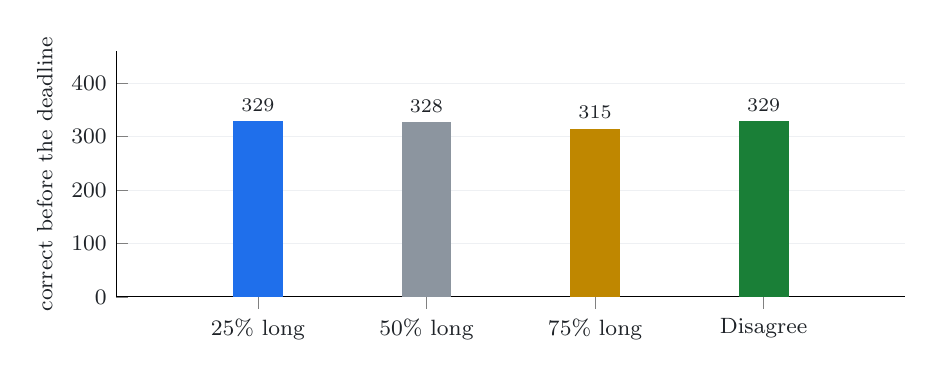
\begin{tikzpicture}
    \begin{axis}[deck, width=11.6cm, height=4.7cm, bar width=18pt,
        ymin=0, ymax=460, ylabel={correct before the deadline},
        ytick={0,100,200,300,400},
        xtick={0,1,2,3},
        xticklabels={{25\% long},{50\% long},{75\% long},{Disagree}}]
      \addplot[fill=accent, draw=none] coordinates {(0,329)};
      \addplot[fill=g2, draw=none] coordinates {(1,328)};
      \addplot[fill=warn, draw=none] coordinates {(2,315)};
      \addplot[fill=good, draw=none] coordinates {(3,329)};
    \end{axis}
  \end{tikzpicture}
  \end{center}
  \src{Practice set, seed 0, one run each. 329/400 is 82.25\%. 328/400 is 82.0\%. 315/400 is 78.75\%.}
\end{frame}

%-------------------------------------------------------------
\begin{frame}{Where the long answer costs the deadline}
  \small
  \renewcommand{\arraystretch}{1.15}
  \begin{tabular}{@{}l r r r r@{}}
    \toprule
    \textbf{Mixture} & \textbf{Correct in time} & \textbf{Started long} & \textbf{Finished in time} & \textbf{Expired} \\
    \midrule
    25\% long & 329 & 94 & 400 & 0 \\
    50\% long & 328 & 187 & 387 & 13 \\
    75\% long & 315 & 298 & 357 & 43 \\
    Disagree & 329 & 69 & 363 & 37 \\
    \bottomrule
  \end{tabular}
  \vspace{0.35em}
  \begin{block}{Reading}
    \small The 25\% rule never misses the clock, and it ties disagree on the score.
    Disagree lets 37 questions expire, then still ties, because it opens the monologue
    only when the short samples cannot agree. The 75\% rule is the one that gives answers away to the deadline.
  \end{block}
  \src{``Started long'' is questions that launched at least one 4{,}096-token monologue.
  Disagree also cancelled 425 samples that were still running; the fraction rules cancelled 0, 35, and 130.}
\end{frame}

%-------------------------------------------------------------
\begin{frame}{What to do with it}
  \begin{exampleblock}{Actionable}
    \small Freeze \textbf{disagree} as the mixture. That is the written rule: same 329 correct-in-time
    answers as 25\% long, and fewer questions sent down the monologue (69 against 94).
    The file is \texttt{selection.json}. It is a practice-set choice, one seed, and the protocol
    already called that choice noisy.
  \end{exampleblock}
  \vspace{0.2em}
  \begin{alertblock}{Not a claim}
    \small Nothing here says a mixture beats always answering short, or always answering long,
    under a deadline. The queue-aware rule was not measured. The 200 fresh questions were not run.
    Seeds 1 and 2 were not run.
  \end{alertblock}
  \vspace{0.2em}
  \begin{block}{The pattern that is safe to repeat}
    \small On this arrival trace, a 4{,}096-token monologue on most of the queue is what misses
    the 4-minute deadline. The missing measurement is the validation list.
  \end{block}
\end{frame}

\end{document}
